\documentclass[a4paper,titlepage,12pt]{article}
\usepackage[dutch]{babel}
\usepackage[utf8]{inputenc}
\usepackage[T1]{fontenc}
\usepackage{lmodern}
\usepackage{graphicx}
\usepackage{hyperref}
\usepackage{url}
\usepackage{listings}
\usepackage{color}
\usepackage{textcomp}
\usepackage{tikz}
\usepackage{titlepic}
\usepackage{float}
\usepackage{multicol}
\usepackage{wrapfig}
\usepackage{caption}

\renewcommand{\familydefault}{\sfdefault}
\renewcommand{\lstlistingname}{Code}


\definecolor{listinggray}{gray}{0.9}
\definecolor{lbcolor}{rgb}{0.9,0.9,0.9}
\definecolor{darkgreen}{rgb}{0.0745,0.568,0.039}
\lstset{
	backgroundcolor=\color{lbcolor},
	tabsize=4,    
	%   rulecolor=,
	language=[GNU]C++,
	basicstyle=\scriptsize,
	upquote=true,
	aboveskip={1.5\baselineskip},
	columns=fixed,
	showstringspaces=false,
	extendedchars=false,
	breaklines=true,
	prebreak = \raisebox{0ex}[0ex][0ex]{\ensuremath{\hookleftarrow}},
	frame=single,
	numbers=left,
	showtabs=false,
	showspaces=false,
	showstringspaces=false,
	identifierstyle=\ttfamily,
	keywordstyle=\color[rgb]{0,0,1},
	commentstyle=\color[rgb]{0.026,0.112,0.095},
	stringstyle=\color[rgb]{0.627,0.126,0.941},
	numberstyle=\color[rgb]{0.205, 0.142, 0.73},
	%        \lstdefinestyle{C++}{language=C++,style=numbers}’.
}
\lstset{
	backgroundcolor=\color{lbcolor},
	tabsize=4,
	language=C++,
	captionpos=b,
	tabsize=3,
	frame=lines,
	numbers=left,
	numberstyle=\tiny,
	numbersep=5pt,
	breaklines=true,
	showstringspaces=false,
	basicstyle=\footnotesize,
	%  identifierstyle=\color{magenta},
	keywordstyle=\color[rgb]{0,0,1},
	commentstyle=\color{darkgreen},
	stringstyle=\color{red}
}

\title{Gamebuino\\ \small{Starters Guide}}
\author{Stijn Caerts}
\titlepic{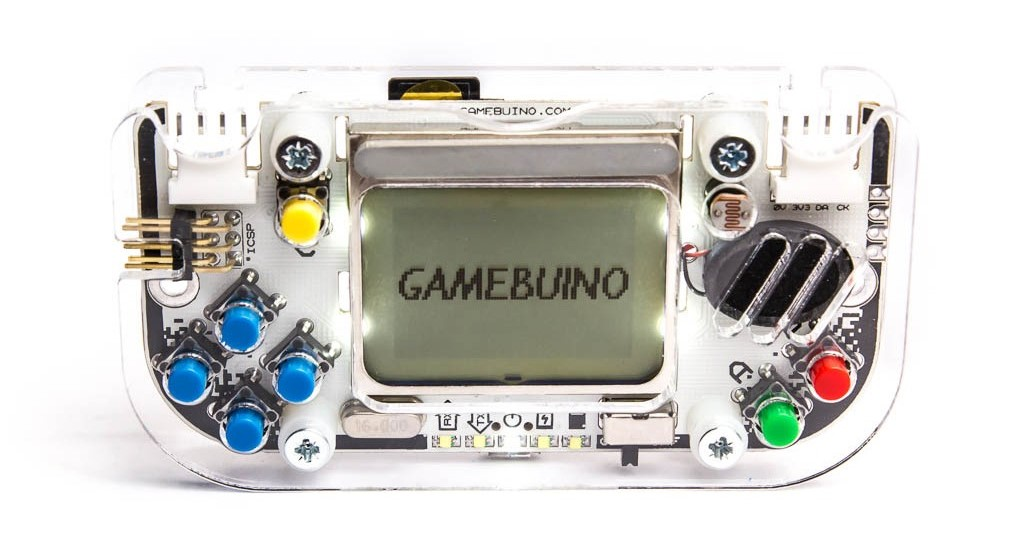
\includegraphics[width=\linewidth]{assets/img/gamebuino-console.jpg}}

\begin{document}
	\begin{titlepage}
		\begin{center}
			
\includegraphics{assets/img/gamebuino_logo.png}
			
			\vspace{0.7cm}
			
			\texttt{Starters Guide}
			
			\vspace{2cm}
			
			Stijn Caerts

			\vspace{2cm}
			
			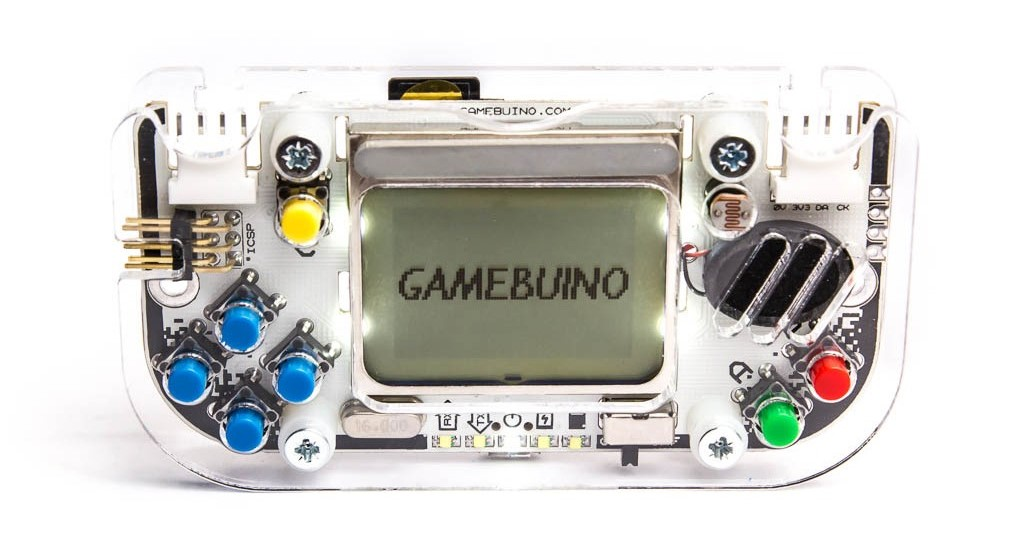
\includegraphics[width=\linewidth]{assets/img/gamebuino-console.jpg}
			
			\vfill
			
			\begin{minipage}{0,45\textwidth}
				\tiny{Augustus 2017}
			\end{minipage}
			\begin{minipage}{0,45\textwidth}
				\begin{flushright}
					
\includegraphics[scale=0.5]{assets/img/JCW.png}
				\end{flushright}
			\end{minipage}
			
		\end{center}
		
		
		
	\end{titlepage}
	\tableofcontents
	\newpage
	
	\section{Basis}
	Net zoals elk programma dat voor Arduino geschreven is, bevat een programma voor Gamebuino de twee functies \texttt{setup()} en \texttt{loop()}. In deze sectie gaan we dieper in op de basisstructuur die in elk programma aanwezig is.
	
	\begin{lstlisting}[language=C++, caption=Structuur van een Gamebuino programma]
	#include <SPI.h>
	#include <Gamebuino.h>
	
	Gamebuino gb;
	
	void setup(){
		gb.begin();
		gb.titleScreen();
		gb.pickRandomSeed();
	}
	
	void loop(){
		if(gb.update()){
			if (gb.buttons.pressed(BTN_C)) {
				gb.titleScreen();
			}
			// GAME
		}
	}
	\end{lstlisting}
	
	
	\subsection{Libraries importeren}
	Voor we aan de slag kunnen gaan met programmeren, moeten we twee libraries importeren. Deze zullen het ons heel wat makkelijker maken om programma's te schrijven voor Gamebuino. De \emph{SPI} library is vereist voor de communicatie met het scherm van de Gamebuino. Verder gebruiken we de \emph{Gamebuino} library, die voor een handige interface zorgt zodat we gemakkelijk alle functies van het apparaat kunnen aanspreken zodat we ons enkel moeten focussen op het ontwerpen en programmeren van het spel zelf.
	Zie wel dat de libraries die je wilt importeren ook geïnstalleerd zijn in de Arduino IDE, anders zal de library niet gevonden worden en zal je de code niet kunnen compilen.
	\begin{lstlisting}[language=C++, caption={Importeren van libraries}]
	#include <SPI.h>
	#include <Gamebuino.h>
	\end{lstlisting}
	
	
	\subsection{Het \texttt{Gamebuino} object}
	Het \texttt{Gamebuino} object heeft een belangrijke plaats in een game. Je zal dit object vaak gebruiken om functies op te roepen die specifiek voor de Gamebuino zijn. De klasse \texttt{Gamebuino} is onderdeel van de \emph{Gamebuino} library.
	\begin{lstlisting}[language=C++, caption={Aanmaken van een \texttt{Gamebuino} object}]
	Gamebuino gb;
	\end{lstlisting}
	
	
	\subsection{\texttt{setup()}}
	De \texttt{setup()} functie wordt eenmaal uitgevoerd bij het opstarten van het programma. Bij een programma voor Gamebuino bevat deze functie steeds de volgende instructies: \texttt{gb.begin()}, \texttt{gb.titleScreen()} en \texttt{gb.pickRandomSeed()}.
	\begin{lstlisting}[language=C++, caption={\texttt{setup()}}]
	void setup(){
		gb.begin();
		gb.titleScreen();
		gb.pickRandomSeed();
	}
	\end{lstlisting}
	
	
	\subsection{\texttt{loop()}}
	De functie \texttt{loop()} bevat de instructies van de game die je gaat programmeren. Deze functie wordt telkens opnieuw uitgevoerd. Om er voor te zorgen dat we ons programma met vaste intervallen uitvoeren, plaatsen we hier een \texttt{if}-statement met \texttt{gb.update()} waarin we alle code van ons programma plaatsen (zoals te zien is in codefragment \ref{code:loop}).
	
	We moeten in ons programma ook steeds de mogelijkheid voorzien om terug te keren naar het titelscherm met de C-knop. Vanuit het titelscherm kan je het spel afsluiten om een ander spel te laden.
	
	\begin{lstlisting}[float=!ht, language=C++, caption={\texttt{loop()}}, label={code:loop}]
	void loop(){
		if(gb.update()){
			if (gb.buttons.pressed(BTN_C)) {
				gb.titleScreen();
			}
			// GAME
		}
	}
	\end{lstlisting}
	
	
	\newpage
	\section{Gamebuino library}
	Hier geven we een overzicht van functies en nuttige variabelen in de \emph{Gamebuino} library.\cite{Gamebuino:Wiki:Reference}
	Optionele argumenten zijn schuingedrukt.
	Voor meer informatie over hoe je deze functies en variabelen kan gebruiken, kan je de voorbeeld-code bekijken in de Arduino IDE via \texttt{File > Examples > Gamebuino}.
	
	\subsection{Core}
	\begin{itemize}
		\item \texttt{gb.begin()}:
		Initialiseer de Gamebuino. Moet éénmaal opgeroepen worden bij het begin van de \texttt{setup()}-functie, gevolgd door \texttt{gb.titleScreen()} en \texttt{gb.pickRandomSeed()}.
		
		\item \texttt{gb.titleScreen(\textit{F("name")}, \textit{logo})}:
		Toon het titelscherm. Moet opgeroepen worden na \texttt{gb.begin()} om het titelscherm te tonen bij het opstarten. Je moet de gebruiker ook toelaten om terug te gaan naar het titelscherm met de C-knop.
		\begin{itemize}
			\item [] \textbf{Parameters}
			\item \textit{F("name")}: Naam die wordt weergegeven op het titelscherm, vervang \textit{name} door de naam van jouw spel.
			\item \textit{\texttt{byte*} logo}: Logo van jouw spel. Kan van formaat variëren tussen 8x8px en 64x30 px, en tot 64x36 px als geen naam is opgegeven.
		\end{itemize}
	
		\item \samepage \texttt{gb.update()}:
		Geeft \texttt{true} en update het display, geluid, batterij monitor, ... met een vaste frequentie (afhankelijk van de frame rate).
		\begin{itemize}
			\item [] \textbf{Return}
			\item \texttt{boolean}: \texttt{true} als voldoende tijd verstreken is sinds het laatste frame.
		\end{itemize}
	
		\item \texttt{gb.setFrameRate(fps)}:
		Pas het aantal frames per seconde aan. Bepaalt hoe vaak per seconde het programma wordt uitgevoerd (zie \texttt{gb.update()}).
		\begin{itemize}
			\item [] \textbf{Parameters}
			\item \texttt{byte} fps: Het aantal frames per seconde, standaard 20 fps.
		\end{itemize}
	
		\item \texttt{gb.pickRandomSeed()}:
		Selecteert een random seed op basis van de batterijspanning, omgevingslicht en de verstreken tijd sinds het opstarten. Moet meteen na \texttt{gb.begin()} en \texttt{gb.titleScreen()} geplaatst worden in \texttt{setup()}.
		
		\item \texttt{gb.changeGame()}:
		Flasht LOADER.HEX van de SD-kaart zodat een ander spel geladen kan worden. Terugkeren naar de loader kan ook via \texttt{gb.titleScreen()}.
		
		\item \texttt{gb.frameCount}:
		Variabele die wordt opgehoogd iedere keer dat er een nieuw frame wordt weergegeven. Aantal frames dat werd gerenderd sinds het programma begon met uitvoeren.
		
		\item \texttt{gb.getDefaultName(name)}:
		Verkrijg de gebruikersnaam die ingesteld is met SETTINGS.HEX.
		\begin{itemize}
			\item [] \textbf{Parameters}
			\item \texttt{char*} name: 10 char lange string waarin de gebruikersnaam wordt opgeslagen.
		\end{itemize}
	\end{itemize}
	
	\subsubsection{User Interface}
	\begin{itemize}
		\item \texttt{gb.menu(menu, length)}:
		Toont een menu met items om uit te kiezen.
		\begin{itemize}
			\item [] \textbf{Parameters}
			\item \texttt{char** PROGMEM} menu: de items waaruit gekozen kan worden, opgeslagen als een \texttt{PROGMEM}-array van strings.
			\item \texttt{byte} length: Aantal items in het menu.
		\end{itemize}
		\samepage
		\begin{itemize}
			\item [] \textbf{Return}
			\item \texttt{char}: Nummer van het geselecteerde item of -1 als het menu verlaten is zonder een item te kiezen.
		\end{itemize}
	
		\item \texttt{gb.keyboard(string, length)}:
		Toon een keyboard zodat de gebruiker tekst kan invoeren.
		\begin{itemize}
			\item [] \textbf{Parameters}
			\item \texttt{char*} string: Ontvangt de tekst ingevoerd door de gebruiker.
			\item \texttt{byte} length: Maximale lengte van de tekst die de gebruiker kan ingeven.
		\end{itemize}
	
		\item \texttt{gb.popup(F("Text"), duration)}: Toon een pop-up melding aan de onderkant van het scherm voor bepaalde duur.
		\begin{itemize}
			\item [] \textbf{Parameters}
			\item \texttt{PROGMEM char*} F("Text"): Tekst die weergegeven moet worden.
			\item \texttt{byte} duration: Hoe lang wordt de pop-up weergegeven, uitgedrukt in aantal frames.
		\end{itemize}
	\end{itemize}
	
	\subsubsection{Physics}
	\begin{itemize}
		\item \texttt{gb.collidePointRect(x1,y1,x2,y2,w,h)}: 
		Controleer of een gegeven punt binnen een rechthoek ligt.
		\begin{itemize}
			\item [] \textbf{Parameters}
			\item \texttt{int} x1: Horizontale coördinaat van het punt.
			\item \texttt{int} y1: Verticale coördinaat van het punt.
			\item \texttt{int} x2: Horizontale coördinaat van de linksboven hoek van de rechthoek.
			\item \texttt{int} y2: Verticale coördinaat van de linksboven hoek van de rechthoek.
			\item \texttt{int} w: Breedte van de rechthoek.
			\item \texttt{int} h: Hoogte van de rechthoek.
		\end{itemize}
		\begin{itemize}
			\item [] \textbf{Return}
			\item \texttt{boolean}: \texttt{true} als het punt binnen de rechthoek ligt, anders \texttt{false}.
		\end{itemize}
	
		\samepage\item \texttt{gb.collideRectRect(x1,y1,w1,h1,x2,y2,w2,h2)}: Controleer of twee rechthoeken snijden of overlappen.
		\begin{itemize}
			\item [] \textbf{Parameters}
			\item \texttt{int} x1: Horizontale coördinaat van de linksboven hoek van de eerste rechthoek.
			\item \texttt{int} y1: Verticale coördinaat van de linksboven hoek van de eerste rechthoek.
			\item \texttt{int} w1: Breedte van de eerste rechthoek.
			\item \texttt{int} h1: Hoogte van de eerste rechthoek.
			\item \texttt{int} x2: Horizontale coördinaat van de linksboven hoek van de tweede rechthoek.
			\item \texttt{int} y2: Verticale coördinaat van de linksboven hoek van de tweede rechthoek.
			\item \texttt{int} w2: Breedte van de tweede rechthoek.
			\item \texttt{int} h2: Hoogte van de tweede rechthoek.
		\end{itemize}
		\begin{itemize}
			\item [] \textbf{Return}
			\item \texttt{boolean}: \texttt{true} als de twee rechthoeken overlappen, anders \texttt{false}.
		\end{itemize}
	
		\item \texttt{gb.collideBitmapBitmap(x1,y1,b1,x2,y2,b2)}: 
		Controleer pixel per pixel of twee bitmaps overlappen.
		\begin{itemize}
			\item [] \textbf{Parameters}
			\item \texttt{int} x1: Horizontale coördinaat van de eerste bitmap.
			\item \texttt{int} y1: Verticale coördinaat van de eerste bitmap.
			\item  \texttt{byte*} b1: Eerste bitmap.
			\item \texttt{int} x2: Horizontale coördinaat van de tweede bitmap.
			\item \texttt{int} y2: Verticale coördinaat van de tweede bitmap.
			\item  \texttt{byte*} b2: Tweede bitmap.
		\end{itemize}
		\begin{itemize}
			\item [] \textbf{Return}
			\item \texttt{boolean}: \texttt{true} als de twee bitmaps overlappen, anders \texttt{false}.
		\end{itemize}
	\end{itemize}

	\subsubsection{Performance monitor}
	\begin{itemize}
		\item \texttt{gb.getCpuLoad()}: Krijg de CPU-belasting uitgedrukt in een percentage.
		\begin{itemize}
			\item [] \textbf{Return}
			\item \texttt{byte}: Percentage van de CPU-tijd die gebruikt wordt. Dit percentage omvat ook de tijd gebruikt door de library voor het updaten van het scherm, audio, schermverlichting, etc.
		\end{itemize}
		
		\item \texttt{gb.getFreeRam()}: Krijg het aantal bytes van het RAM-geheugen dat vrij is door de afstand tussen de heap en de stack te meten. Resultaat is niet consistent.
		\begin{itemize}
			\item [] \textbf{Return}
			\item \texttt{int}: Aantal bytes van het RAM-geheugen dat vrij is. 
		\end{itemize}
		
		\item  \texttt{gb.frameDurationMicros}: Tijd die nodig was om het laatste frame te renderen, uitgedrukt in microsecondes.
	\end{itemize}

	\subsection{Buttons}
	De verschillende knoppen die aanwezig zijn op een Gamebuino, staan in de library als een constante. Via deze constantes kan je eenvoudig verwijzen naar een bepaalde knop, zonder de overeenkomstige \texttt{byte} te moeten ingeven.
	
	De beschikbare knoppen zijn:
	\begin{multicols}{4}
		\begin{itemize}
			\item \texttt{BTN\_UP}
			\item \texttt{BTN\_DOWN}
			\item \texttt{BTN\_LEFT}
			\item \texttt{BTN\_RIGHT}
			\item \texttt{BTN\_A}
			\item \texttt{BTN\_B}
			\item \texttt{BTN\_C}
		\end{itemize}
	\end{multicols}

	Er zijn verschillende functies om met de knoppen te interageren.
	\begin{itemize}
		\item \texttt{gb.buttons.pressed(button)}: 
		Gebruikt om te weten wanneer een knop ingedrukt wordt.
		\begin{itemize}
			\item [] \textbf{Parameters}
			\item \texttt{byte} button: Identifier van de knop.
		\end{itemize}
		\begin{itemize}
			\item [] \textbf{Return}
			\item \texttt{boolean}:  \texttt{true} als de knop ingedrukt wordt, anders \texttt{false}.
		\end{itemize}
	
		\samepage\item \texttt{gb.buttons.released(button)}: Gebruikt om te weten wanneer een knop losgelaten wordt.
		\begin{itemize}
			\item [] \textbf{Parameters}
			\item \texttt{byte} button: Identifier van de knop.
		\end{itemize}
		\begin{itemize}
			\item [] \textbf{Return}
			\item \texttt{boolean}: \texttt{true} als de knop losgelaten wordt, anders \texttt{false}.
		\end{itemize}
	
		\item \texttt{gb.buttons.held(button, duration)}: Gebruikt om te weten wanneer een knop voor een bepaalde tijd ingedrukt wordt.
		\begin{itemize}
			\item [] \textbf{Parameters}
			\item \texttt{byte} button: Identifier van de knop.
			\item \texttt{byte} duration: Duur in aantal frames.
		\end{itemize}
		\begin{itemize}
			\item [] \textbf{Return}
			\item \texttt{boolean}: \texttt{true} als de knop ingedrukt is voor het gegeven aantal frames, anders \texttt{false}. Geeft slechts eenmaal \texttt{true} terug.
		\end{itemize}
	
		\item \texttt{gb.buttons.repeat(button, duration)}: Gebruikt om een actie te herhalen met een vast interval zolang een knop ingedrukt wordt.
		\begin{itemize}
			\item [] \textbf{Parameters}
			\item \texttt{byte} button: Identifier van de knop.
			\item \texttt{byte} duration: Duur in aantal frames.
		\end{itemize}
		\begin{itemize}
			\item [] \textbf{Return}
			\item \texttt{boolean}: \texttt{true} iedere keer dat het gegeven aantal frames is gepasseerd zolang de knop ingedrukt wordt, anders \texttt{false}.
		\end{itemize}
	
		\item \texttt{gb.buttons.timeHeld(button)}: Gebruikt om te weten hoe lang een knop ingedrukt wordt.
		\begin{itemize}
			\item [] \textbf{Parameters}
			\item \texttt{byte} button: Identifier van de knop.
		\end{itemize}
		\begin{itemize}
			\item [] \textbf{Return}
			\item \texttt{byte}: Aantal frames dat de knop ingedrukt is.
		\end{itemize}
	\end{itemize}


	\subsection{Display}
	\subsubsection{Constants}
	\begin{itemize}
		\item \texttt{LCDWIDTH}: Breedte van het scherm in pixels.
		\item \texttt{LCDHEIGHT}: Hoogte van het scherm in pixels.
		\item \texttt{gb.display.fontWidth}: Breedte van het huidige font.
		\item \texttt{gb.display.fontHeight}: Hoogte van het huidige font.
	\end{itemize}

	\subsubsection{General}
	\begin{itemize}
		\item \texttt{gb.display.persistence} \texttt{(boolean)}: Kies om het scherm te wissen tussen elk frame (\texttt{false}) of niet (\texttt{true}). Standaardwaarde is \texttt{false}.
		
		\item \texttt{gb.display.clear()}: Wis de display buffer en stel de positie van de tekstcursor in op $(0,0)$. Als het scherm tussen elk frame gewist moet worden, gebruik dan \texttt{gb.display.persistence}.
		
		\item \texttt{gb.display.update()}: Stuur de display buffer naar het display. Gebeurt elk frame automatisch met \texttt{gb.update()}, dus je moet deze functie niet zelf oproepen.
		
		\item \texttt{gb.display.fillScreen(color)}: Vul het volledige scherm met een kleur.
		\begin{itemize}
			\item [] \textbf{Parameters}
			\item \texttt{byte} color: \texttt{BLACK} of \texttt{WHITE}.
		\end{itemize}
		
		\item \texttt{gb.display.setColor(foreground, \textit{background})}: Verander de kleur die gebruikt wordt om te tekenen op het scherm. Mogelijke kleuren zijn: \texttt{WHITE}, \texttt{BLACK}, \texttt{GRAY} en \texttt{INVERT}.
		\begin{itemize}
			\item [] \textbf{Parameters}
			\item \texttt{byte} foreground: Kleur van de voorgrond.
			\item \textit{\texttt{byte} background}: Kleur van de achtergrond. Als de achtergrondkleur niet gespecificeerd is, dan is de achtergrond transparant.
		\end{itemize}
	\end{itemize}

	\subsubsection{Pixels}
	\begin{itemize}
		\item \texttt{gb.display.drawPixel(x, y)}: Teken één pixel op de gegeven coördinaten. Kleur wordt bepaald door \texttt{gb.display.setColor()}
		\begin{itemize}
			\item [] \textbf{Parameters}
			\item \texttt{byte} x: Horizontale coördinaat, tussen $0$ en \texttt{LCDWIDTH}.
			\item \texttt{byte} y: Verticale coördinaat, tussen $0$ en \texttt{LCDHEIGHT}.
		\end{itemize}
	
		\item \texttt{gb.display.getPixel(x, y)}: Verkrijg de kleur van de gevraagde pixel.
		\begin{itemize}
			\item [] \textbf{Parameters}
			\item \texttt{byte} x: Horizontale coördinaat.
			\item \texttt{byte} y: Verticale coördinaat.
		\end{itemize}
		\begin{itemize}
			\item [] \textbf{Return}
			\item \texttt{byte}: $0$ voor \texttt{WHITE}, $1$ voor \texttt{BLACK}.
		\end{itemize}
	\end{itemize}

	\subsubsection{Lines}
	\begin{itemize}
		\item \texttt{gb.display.drawLine(x1,y1,x2,y2)}: Tekent een rechte lijn van een punt naar een ander punt.
		\begin{itemize}
			\item [] \textbf{Parameters}
			\item \texttt{byte} x1: Horizontale coördinaat van het eerste punt.
			\item \texttt{byte} y1: Verticale coördinaat van het eerste punt.
			\item \texttt{byte} x2: Horizontale coördinaat van het tweede punt.
			\item \texttt{byte} y2: Verticale coördinaat van het tweede punt.
		\end{itemize}
	
		\item \texttt{gb.display.drawFastVLine(x,y,h)}: Teken een verticale lijn.
		\begin{itemize}
			\item [] \textbf{Parameters}
			\item \texttt{byte} x: Horizontale coördinaat van het beginpunt.
			\item \texttt{byte} y: Verticale coördinaat van het beginpunt.
			\item \texttt{byte} h: Lengte (hoogte) van de lijn.
		\end{itemize}
	
		\item \texttt{gb.display.drawFastHLine(x,y,w)}: Teken een verticale lijn.
		\begin{itemize}
			\item [] \textbf{Parameters}
			\item \texttt{byte} x: Horizontale coördinaat van het beginpunt.
			\item \texttt{byte} y: Verticale coördinaat van het beginpunt.
			\item \texttt{byte} w: Lengte (breedte) van de lijn.
		\end{itemize}
	\end{itemize}

	\subsubsection{Rectangles}
	\begin{itemize}
		\item \texttt{gb.display.drawRect(x,y,w,h)}: Teken een rechthoek.
		\begin{itemize}
			\item [] \textbf{Parameters}
			\item \texttt{byte} x: Horizontale coördinaat van de linksboven hoek.
			\item \texttt{byte} y: Verticale coördinaat van de linksboven hoek.
			\item \texttt{byte} w: Breedte van de rechthoek.
			\item \texttt{byte} h: Hoogte van de rechthoek.
		\end{itemize}
	
		\item \texttt{gb.display.fillRect(x,y,w,h)}: Teken en vul een rechthoek.
		\begin{itemize}
			\item [] \textbf{Parameters}
			\item \texttt{byte} x: Horizontale coördinaat van de linksboven hoek.
			\item \texttt{byte} y: Verticale coördinaat van de linksboven hoek.
			\item \texttt{byte} w: Breedte van de rechthoek.
			\item \texttt{byte} h: Hoogte van de rechthoek.
		\end{itemize}
	
		\item \texttt{gb.display.drawRoundRect(x,y,w,h,r)}: Teken een rechthoek met afgeronde hoeken.
		\begin{itemize}
			\item [] \textbf{Parameters}
			\item \texttt{byte} x: Horizontale coördinaat van de linksboven hoek.
			\item \texttt{byte} y: Verticale coördinaat van de linksboven hoek.
			\item \texttt{byte} w: Breedte van de rechthoek.
			\item \texttt{byte} h: Hoogte van de rechthoek.
			\item \texttt{byte} r: Afronding van de hoeken.
		\end{itemize}
	
		\item \texttt{gb.display.fillRoundRect(x,y,w,h,r)}: Teken en vul een rechthoek met afgeronde hoeken.
		\begin{itemize}
			\item [] \textbf{Parameters}
			\item \texttt{byte} x: Horizontale coördinaat van de linksboven hoek.
			\item \texttt{byte} y: Verticale coördinaat van de linksboven hoek.
			\item \texttt{byte} w: Breedte van de rechthoek.
			\item \texttt{byte} h: Hoogte van de rechthoek.
			\item \texttt{byte} r: Afronding van de hoeken.
		\end{itemize}
	\end{itemize}

	\subsubsection{Circles}
	\begin{itemize}
		\item \texttt{gb.display.drawCircle(x,y,r)}: Teken een cirkel.
		\begin{itemize}
			\item [] \textbf{Parameters}
			\item \texttt{byte} x: Horizontale coördinaat van het middelpunt van de cirkel.
			\item \texttt{byte} y: Verticale coördinaat van het middelpunt van de cirkel.
			\item \texttt{byte} r: Straal van de cirkel.
		\end{itemize}
	
		\item \texttt{gb.display.fillCircle(x,y,r)}: Teken en vul een cirkel.
		\begin{itemize}
			\item [] \textbf{Parameters}
			\item \texttt{byte} x: Horizontale coördinaat van het middelpunt van de cirkel.
			\item \texttt{byte} y: Verticale coördinaat van het middelpunt van de cirkel.
			\item \texttt{byte} r: Straal van de cirkel.
		\end{itemize}
	\end{itemize}


	\subsubsection{Triangles}
	\begin{itemize}
		\item \texttt{gb.display.drawTriangle(x1,y1,x2,y2,x3,y3)}: Teken een driehoek.
		\begin{itemize}
			\item [] \textbf{Parameters}
			\item \texttt{byte} x1: Horizontale coördinaat van de eerste hoek.
			\item \texttt{byte} y1: Verticale coördinaat van de eerste hoek.
			\item \texttt{byte} x2: Horizontale coördinaat van de tweede hoek.
			\item \texttt{byte} y2: Verticale coördinaat van de tweede hoek.
			\item \texttt{byte} x3: Horizontale coördinaat van de derde hoek.
			\item \texttt{byte} y3: Verticale coördinaat van de derde hoek.
		\end{itemize}
	
		\item \texttt{gb.display.fillTriangle(x1,y1,x2,y2,x3,y3)}: Teken en vul een driehoek.
		\begin{itemize}
			\item [] \textbf{Parameters}
			\item \texttt{byte} x1: Horizontale coördinaat van de eerste hoek.
			\item \texttt{byte} y1: Verticale coördinaat van de eerste hoek.
			\item \texttt{byte} x2: Horizontale coördinaat van de tweede hoek.
			\item \texttt{byte} y2: Verticale coördinaat van de tweede hoek.
			\item \texttt{byte} x3: Horizontale coördinaat van de derde hoek.
			\item \texttt{byte} y3: Verticale coördinaat van de derde hoek.
		\end{itemize}
	\end{itemize}

	\subsubsection{Bitmaps}
	\begin{itemize}
		\item \texttt{gb.display.drawBitmap(x, y, bitmap, \textit{rotation}, \textit{flip})}: Teken een bitmap gegeven als een byte array op het scherm.
		\begin{itemize}
			\item [] \textbf{Parameters}
			\item \texttt{byte} x: Horizontale coördinaat op het scherm.
			\item \texttt{byte} y: Verticale coördinaat op het scherm.
			\item \texttt{byte} bitmap: Een byte array.
			\item \textit{\texttt{byte} rotation}: Rotatie: \texttt{NOROT}, \texttt{ROTCW}, \texttt{ROTCCW} of \texttt{ROT180}.
			\item \textit{\texttt{byte} flip}: Spiegeling: \texttt{NOFLIP}, \texttt{FLIPH}, \texttt{FLIPV} of \texttt{FLIPVH}.
		\end{itemize}
	\end{itemize}

	\subsubsection{Text}
	\begin{minipage}{.75\textwidth}
		\begin{itemize}
			\item \texttt{gb.display.print(data)}: Print data op het scherm.
			\begin{itemize}
				\item [] \textbf{Parameters}
				\item data: De data die geprint moet worden. Kan verscheidene datatypes hebben. Om RAM-geheugen te sparen, kan je een string uit het flash-memory doorgeven met \texttt{F(data)}.
			\end{itemize}
		
			\item \texttt{gb.display.println(data)}: Print data op het scherm, gevolgd door een carriage return (\texttt{\textbackslash r}) en newline (\texttt{\textbackslash n}) karakter.
			\begin{itemize}
				\item [] \textbf{Parameters}: zie \texttt{gb.display.print()}
			\end{itemize}
		
			\item \texttt{gb.display.drawChar(x, y, c, s)}: Teken een karakter op de opgegeven plaats.
			\begin{itemize}
				\item [] \textbf{Parameters}
				\item \texttt{byte} x: Horizontale coördinaat.
				\item \texttt{byte} y: Verticale coördinaat.
				\item \texttt{char} c: Code van karakter in de tabel (zie Figuur \ref{fig:characterTable}).
				\item \texttt{byte} s: Grootte van het karakter.
			\end{itemize}
		\end{itemize}
	\end{minipage}
	\hspace{0.05\textwidth}
	\begin{minipage}{.20\textwidth}
		\centering
		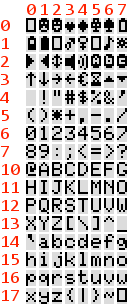
\includegraphics[scale=0.6]{assets/img/font5x7}
		\captionof{figure}{\label{fig:characterTable}Beschikbare karakters in het standaard font.}
	\end{minipage}

	\begin{itemize}
		\item \samepage \texttt{gb.display.setFont(font)}: Verander het font dat gebruikt wordt om tekst te weergeven. \\ Er zijn drie varianten van het standaard font: \emph{font3x3}, \emph{font3x5} en \emph{font5x7}. Om één van de standaard fonts te gebruiken, moet je het volgende toevoegen: \texttt{extern const byte font5x7[];} waarbij je de naam van het gewenste font invult.
		\begin{itemize}
			\item [] \textbf{Parameters}
			\item \texttt{byte*} font: Lettertype.
		\end{itemize}
	
		\item \texttt{gb.display.cursorX}: Horizontale coördinaat van de cursor.
		\item \texttt{gb.display.cursorY}: Verticale coördinaat van de cursor.
		
		\item \texttt{gb.display.fontSize}: De grootte van het font. Gebruikt om te schalen, standaardwaarde is $1$.
		
		\item \texttt{gb.display.textWrap}: Kies of de tekst aan de rechterkant van het scherm wordt afgebroken of niet.
	\end{itemize}

	\subsection{Sound}
	Voor een uitgebreider overzicht van de beschikbare functies kan je de Gamebuino Wiki\cite{Gamebuino:Wiki:Reference} raadplegen.
	\begin{itemize}
		\item \texttt{gb.sound.playOK()}
		\item \texttt{gb.sound.playCancel()}
		\item \texttt{gb.sound.playTick()}
	\end{itemize}

	\subsection{Battery}
	\begin{itemize}
		\item \texttt{gb.battery.voltage}: Spanning van de batterij in mV.
		
		\item \texttt{gb.battery.level}: Batterijniveau, ingedeeld volgens de drempels in \emph{SETTINGS.HEX}.
		
		\item \texttt{gb.battery.show}: Kies of de batterij indicator weergegeven wordt.
	\end{itemize}

	\newpage
	\section{Testen}
	Als je een game aan het programmeren bent, wil je natuurlijk ook kunnen testen of deze werkt op de manier dat jij wil. De game iedere keer op de SD-kaart plaatsen als je aanpassingen hebt gemaakt is een tijdrovend proces en daarom niet de ideale manier om snel iets te testen.
	
	Om deze reden bestaan er Gamebuino emulators\cite{Gamebuino:Wiki:Emulators}, die de werking van een Gamebuino nabootsen op de computer. Er zijn verschillende emulators beschikbaar, maar Simbuino4Web (\url{http://simbuino4web.ppl-pilot.com/}) is het eenvoudigst om te gebruiken omdat het geen installatie vereist. \\
	
	Voordat je de emulator kan gebruiken, moet je eerst jouw game compileren in de Arduino IDE. Dit doe je als volgt: \texttt{Sketch > Export compiled Binary}. Vervolgens kan je dan het gecompileerde bestand, \emph{Game.ino.standard.hex}, gebruiken in de emulator.
	
	\begin{figure}[!b]
		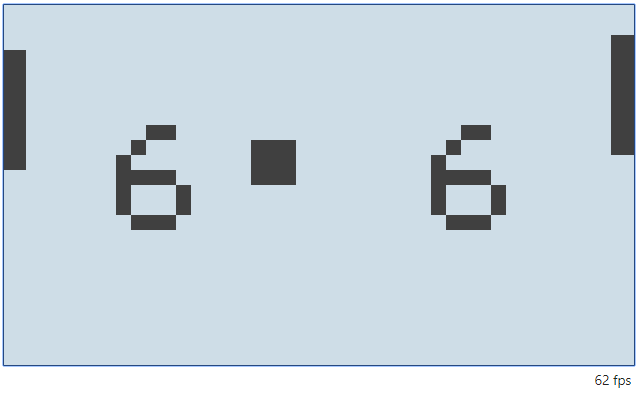
\includegraphics[width=\textwidth]{assets/img/Simbuino4Web.png}
		\caption{Simbuino4Web}
	\end{figure}
	
	
	\newpage
	\section{Programma op Gamebuino plaatsen}
	De Gamebuino laadt bij het opstarten een bootloader, het menu waar je verschillende spelletjes kan kiezen. Om je eigen programma in deze lijst weer te geven, moet je het gecompileerde programma op de SD-kaart plaatsen. Het gecompileerde programma is een bestand met als extensie \emph{.hex}. Dit bestand moet je hernoemen zodat de naam enkel hoofdletters bevat en een maximale lengte heeft van 8 karakters voor de extensie, zoals in Figuur \ref{fig:hernoemen}.
	\begin{figure}[h]
		\centering
		\fbox{
			\parbox{8cm}{
				\centering
				Pong.hex \(\longrightarrow\) PONG.HEX \\
				SpaceInvaders.hex \(\longrightarrow\) SPACEINV.HEX
			}
		}
		\caption{\label{fig:hernoemen}Hernoemen van gecompileerde programma's}
	\end{figure}
	
	% INF encoder
	Als je wil dat jouw game met logo en beschrijving wordt weergegeven in het menu, moet je ook een \emph{.INF}-bestand maken met dezelfde naam. Dit doe je met een \textbf{INF encoder}\cite{GitHub:Rodot:InfEncoder}. Deze encoder zet die informatie om naar een bestand dat de Gamebuino-loader kan lezen. Hiervoor heb je een logo nodig van 19x18 px en je kan tot 255 slides van 84x32 px toevoegen die meer vertellen over de game. De afbeeldingen die je gebruikt voor het logo of de slides mogen enkel de kleuren wit en zwart bevatten, daarom kan je hiervoor best een monochrome bitmap gebruiken als bestandsformaat.
	
	Nu heb je twee bestanden met dezelfde naam en de extensies \emph{.HEX} en \emph{.INF}. Door deze twee bestanden op de SD-kaart te plaatsen, zal jouw eigen game nu ook in het opstartmenu verschijnen!
	
	\begin{figure}[!ht]
		\centering
		\fbox{
\includegraphics[height=3cm]{assets/img/icon}}
		\fbox{
\includegraphics[height=3cm]{assets/img/slide1}}
		\caption{\label{fig:logo_slide}Voorbeeld van een logo en slide voor Pong, \textbf{niet} op gelijke schaal}
	\end{figure}
	
	\newpage
	\bibliographystyle{unsrt}
	\bibliography{document}
\end{document}